\documentclass[12pt,aspectratio=43]{beamer}

% 自訂字體的封包
\usepackage{fontspec}

% 導入圖形與表格的封包
\usepackage{graphicx}
\graphicspath{{./20251231_Meeting}}

\usepackage{booktabs}

% 排列多個子圖形的封包
\usepackage{subfigure} 

 % 提供進階數學環境與公式排版
\usepackage{mathtools, amsmath, amsfonts, amsthm, latexsym}

%% 設定中文字體
\usepackage{xeCJK}
\setCJKmainfont[AutoFakeBold=3.5 , AutoFakeSlant=0.2]{標楷體}
\setmainfont{Times New Roman}
\XeTeXlinebreaklocale "zh"
\XeTeXlinebreakskip = 0pt plus 1pt

% 自訂字體顏色的封包
\usepackage{color} 

% 圖表自動編號的封包
\usepackage{caption} 

% 允許表格的一格能多列呈現的封包
\usepackage{multirow} 

% 可指定表格排版的封包
\usepackage{array}

% 翻轉表格的封包
\usepackage{lscape} 

% 序列標號
\usepackage{enumerate} 

%% 設定自動編號
\setbeamertemplate{caption}[numbered]

%% 自訂顏色
\definecolor{Myblue}{RGB}{57,108,144}
\definecolor{Default_Blue}{RGB}{52,51,171}

% (動畫)字會若隱若現的顯示
\beamersetuncovermixins{\opaqueness<1->{45}}{\opaqueness<1->{95}} 

% 設定中文的標籤
\renewcommand{\figurename}{圖} 
\renewcommand{\tablename}{表} 

% 排版形式 
\mode<presentation>{
\usetheme{Berlin}
% enumerate 及 item 的形狀
\setbeamertemplate{itemize items}[triangle]
% 調整外框形式的字體大小
\setbeamerfont{headline}{size=\scriptsize}
\setbeamerfont{footline}{size=\scriptsize}
% 取消右下方的跳轉工具列
\setbeamertemplate{navigation symbols}{} 
% 自定義2：清除外框下緣但僅出頁碼
\setbeamertemplate{footline}[page number] 
% 顏色主題
\usecolortheme{dove}
% 設定頁面邊界
\setbeamersize{text margin left=0.6cm, text margin right=0.6cm}
\special{papersize=\the\paperwidth,\the\paperheight}
\providecommand{\tabularnewline}{\\}
}

\title{Meeting 1231}
\author{黃丞暘}
\institute{國立東華大學應數統計所}
\date{December 31, 2025}

\begin{document}

% 封面
\begin{frame}
  \titlepage
\end{frame}

% 目錄
\begin{frame}{\textbf{Index}}
  \tableofcontents
\end{frame}

% DISCUSSION 
\section{12.31 Discussion}

\begin{frame}{\textbf{12.31 Discussion}}
\linespread{1.5}
Semiconductor Manufacturing Process

  \begin{itemize}
    \item \textbf{Unbox black-box function $\hat f$}
    \begin{enumerate}[]
      \item 在PCA平面（有拿掉極端值），clusters內的0/1有可分性  
      \item 選定「有故事的」 $X_0$作為敘事地標（landmark）
      \item 上次有用 $X_{\text{test}}$，下次可選擇 $\hat p(x|x \in X_0)\approx 0.5$ 的點
    \end{enumerate}

    \item \textbf{Decision strategy}
    \begin{enumerate}[]
      \item fail來自FAR低的cluster $\Rightarrow$ 高可信度的fail
      \item fail來自FAR高的cluster $\Rightarrow$ 需優先調查該cluster
    \end{enumerate}
  \end{itemize}
\end{frame}

\begin{frame}{\textbf{12.31 Discussion}}
\linespread{1.5}

\begin{itemize}
  \item \textbf{討論 local $R^2$ 與 $\hat p(x_0)$ 的關係}
  \begin{enumerate}[]
    \item local $R^2$ 衡量的是 local surrogate $\hat{\hat{g}}$對黑箱 $\hat f$ 的局部擬合度
    \item 因此 $\hat p(x_0)\approx 0.5$ 時的 local $R^2$ 很高並不矛盾；若在 $\hat p(x_0)\to 0/1$ （黑箱更確定時）， local $R^2$ 下降，表示目前的局部模型$\hat{\hat{g}}$在那些區域不足以逼近$\hat{f}$，需要更強的$\hat{\hat{g}}$
  \end{enumerate}
\end{itemize}

\end{frame}

% TO DO
\section{12.31 Todo}

\begin{frame}{\textbf{12.31 Todo}}
\linespread{1.5}
  \begin{itemize}
    \item \textbf{Separate and fit black-box function}
    \begin{enumerate}[]
      \item 將資料切分：$\mathcal{D}_c=\{(x_i, y_i):c_i=c\}$，其中$c \in \{1,...,K\}$，
      對每個 cluster 獨立訓練 black-box $\hat{f}_c:x\longmapsto\hat{p}_c(x)$
    \end{enumerate}
  \end{itemize}

  \begin{itemize}
    \item \textbf{Choose other $x_0$}
    \begin{enumerate}[]
      \item 選擇 $\hat p(x_0)\approx 0.5$ 的點，作為local的解釋地標
      \item 對$x_0$做local surrogate（生成$x_{\ell}=x_0+\varepsilon_{\ell}$），計算$y_{\ell}=\hat{f}_c(x_{\ell})$
      ，最後fit模型$\hat{\hat{g}}$
    \end{enumerate}
  \end{itemize}

  \begin{itemize}
    \item \textbf{Try other ML as $\hat{\hat g}$}
    \begin{enumerate}[]
      \item 使用Logistic作為black-box，XGBoost作為$\hat{\hat g}$
    \end{enumerate}
  \end{itemize}
\end{frame}

% 結果
\section{Results - What I did this time}

\begin{frame}{\textbf{Results I}　{SMOTE + PCA + KMeans}}
\linespread{0.9}

\begin{center}
  \begin{minipage}{0.45\linewidth}
    \centering
    
\includegraphics[width=\linewidth]{pca.png}
  \end{minipage}
  \hspace{0.3em}
  \begin{minipage}{0.45\linewidth}
    \centering
    
\includegraphics[width=\linewidth]{pca2.png}
  \end{minipage}
\end{center}

\small{$$
\begin{array}{c|cc}
\text{cluster} & 0 & 1 \\
\hline
y=0 & 743 & 687 \\
y=1 & 205 & 510 \\
\end{array}
$$}

\end{frame}

\begin{frame}{\textbf{Results II} {Build a surrogate model}}
\linespread{1.5}
Reference: \href{https://ucinlp.github.io/files/papers/lime-naacl16demo.pdf}{Ribeiro et al.(2016)}
  \begin{itemize}
    \item 給定一個設計點 $x_0$
    \item 生成局部擾動樣本：$x_{\ell}=x_0+\varepsilon_{\ell}$，其中 $\varepsilon_{\ell}\sim N(0,\sigma^2 I)$
    \item 代入對應的 cluster black-box：$y_{\ell}=\hat f_c(x_{\ell})$
    \item 以 $\{(x_{\ell},y_{\ell})\}$ 擬合簡單的 local surrogate $\hat{\hat g}$，
          使得在 $x_0$ 鄰域內 $\hat f_c(x)\approx \hat{\hat g}(x;x_0)$
  \end{itemize}
\end{frame}

\begin{frame}{\textbf{Results II}　{SMOTE}}

\begin{center}
  \begin{minipage}{0.35\linewidth}
    \centering
    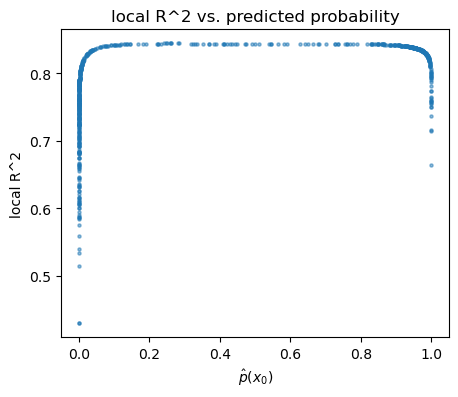
\includegraphics[width=\linewidth]{localpvsR1.png} 
    $\hat{f}$ is logistic\\
    $\hat{\hat{g}}$ is linear
  \end{minipage}
  \hspace{0.3em}
  \begin{minipage}{0.35\linewidth}
    \centering
    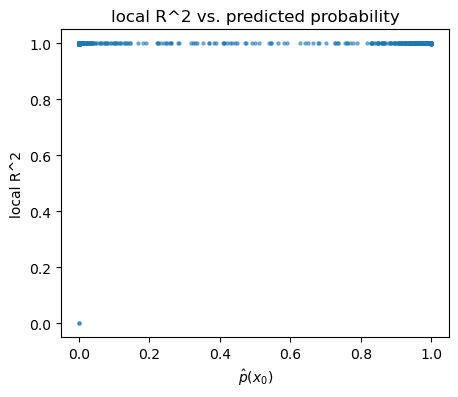
\includegraphics[width=\linewidth]{f_XGB&g_logistic.png}
    $\hat{f}$ is logistic\\
    $\hat{\hat{g}}$ is XGBoost
  \end{minipage}
\end{center}

\end{frame}

% --- 結束 ---
\section*{結束}

\begin{frame}[plain] % 產生無外框的頁面
	\begin{center}
		{\Huge The End}
		\bigskip\bigskip 

		{\LARGE Questions  \&  Comments}
	\end{center}
\end{frame}
\end{document}ㄒ
